\documentclass[a4paper]{article}
\usepackage[utf8]{inputenc}
\usepackage[T1]{fontenc}
\usepackage[french]{babel}
\usepackage{amsmath, amssymb}
\usepackage{graphicx}
\usepackage{hyperref}
\usepackage{geometry}
\geometry{margin=2.5cm}
	\title{Projet BJT EISC Partie 1}
\author{Votre Nom}
\date{2026-02-11}
\begin{document}
\maketitle
\begin{center}
	
\includegraphics[width=0.4\textwidth]{ProjetBJTEISCPartie1202-img/ProjetBJTEISCPartie1202-img001.png} \\
		\textbf{Année Universitaire 2025-2026}
\end{center}
\begin{center}
	\begin{tabular}{c c}
		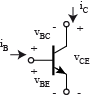
\includegraphics[width=0.2\textwidth]{ProjetBJTEISCPartie1202-img/ProjetBJTEISCPartie1202-img003.png} &
		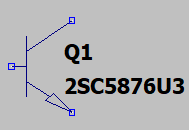
\includegraphics[width=0.2\textwidth]{ProjetBJTEISCPartie1202-img/ProjetBJTEISCPartie1202-img004.png} \\
		Symbole du transistor NPN & Transistor 2SC5876U3 : élément LTspice \\
	\end{tabular}
\end{center}

\section*{Introduction à LTspice}
LTspice est un simulateur circuit basé sur le standard \textbf{SPICE}, développé par la société Analog Devices. Cet outil logiciel gratuit n’a pas de limitation sur le nombre de nœuds ou de composants, c’est un standard de l'industrie pour la simulation de circuits analogiques. Pour analyser ou concevoir un circuit, c'est un outil indispensable qui permet de passer d'un schéma théorique à une visualisation précise des signaux électriques (tensions, courants, spectres de fréquence) avant d’envisager un premier prototype.

Pour télécharger le logiciel LTspice, rendez-vous sur :
\url{https://www.analog.com/en/resources/design-tools-and-calculators/ltspice-simulator.html}

Pour la prise en main du logiciel, rendez-vous sur le LT wiki :
\url{https://ltwiki.org/}

\section*{Introduction du projet}
L'objectif du projet est de réaliser à l'aide du logiciel LTspice les études statique et dynamique de différents montages intégrant un transistor bipolaire de type NPN 2SC5876U3 de la société Rohm semiconductor. Toutes les informations sur le composant sont disponibles au lien suivant :
\url{https://www.rohm.com/products/transistors/bipolar-transistors/automotive-bipolar-transistors/2sc5876u3hzg-product#productDetail}

\section*{PARTIE 1 : Caractérisation du transistor}
\begin{itemize}
	\item $I_C = f(I_B)$
	\item $I_C = f(V_{CE})$
	\item $V_{BE}=f(I_{B})$
	\item $V_{BE}=f(V_{CE})$
\end{itemize}
Note : Pour $I_{C}=f(V_{CE})$ on choisira 3 à 4 valeurs de $I_{B}$ dans la gamme de compatibilité du transistor.

Pour cela une possibilité est l’utilisation du montage de la figure 1 et du mode de simulation \texttt{.DC sweep}.
\begin{center}
	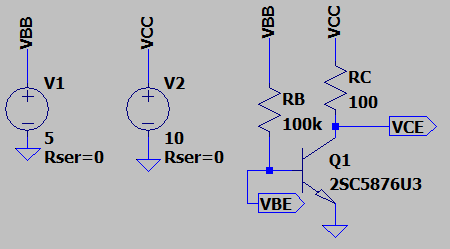
\includegraphics[width=0.5\textwidth]{ProjetBJTEISCPartie1202-img/ProjetBJTEISCPartie1202-img005.png} \\
		extit{Figure 1 : Montage d’analyse des caractéristiques du transistor}
\end{center}
Q1. En détailler votre démarche de simulation, tracer chacune des caractéristiques du transistor et repérer les zones de fonctionnement du transistor. À partir de l’analyse des courbes obtenues, vérifier l’adéquation entre les résultats de simulation, la documentation technique et les paramètres du modèle SPICE du composant.

Pour tracer les courbes suivantes $I_C=f(I_B)$, $I_C=f(V_{CE})$, $V_{BE}=f(I_B)$, $V_{BE}=f(V_{CE})$, nous commençons par créer un projet sur LTspice et réaliser le montage de la Figure 1.

\subsection*{Caractéristique Gain Courant : $I_C=f(I_B)$}
Pour cette caractéristique, il faut :
\begin{itemize}
	\item Effectuer un DC sweep sur la source de tension $V_1$ qui alimente $V_{BB}$ (contrôle $I_B$ via $R_B$)
	\item Utiliser une source continue simple pour $V_2$
\end{itemize}
\begin{center}
	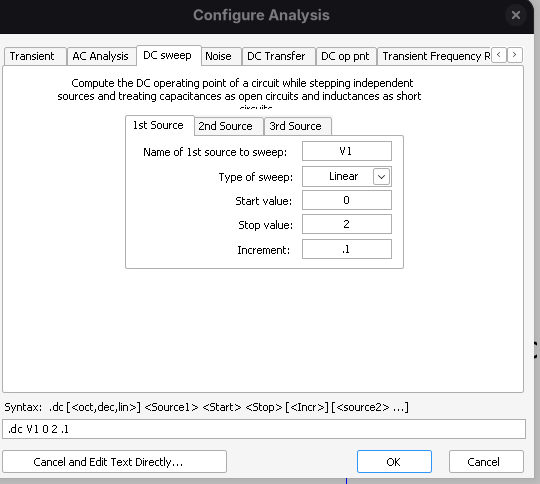
\includegraphics[width=0.4\textwidth]{ProjetBJTEISCPartie1202-img/ProjetBJTEISCPartie1202-img006.png} \\
	Montage LTspice pour $I_C=f(I_B)$
\end{center}
Pour tracer la caractéristique $I_C=f(I_B)$, il faut tracer $I_C(Q1)$ ou $I(R_C)$ sur l’axe Y et $I(R_B)$ sur l’axe X.
\begin{center}
	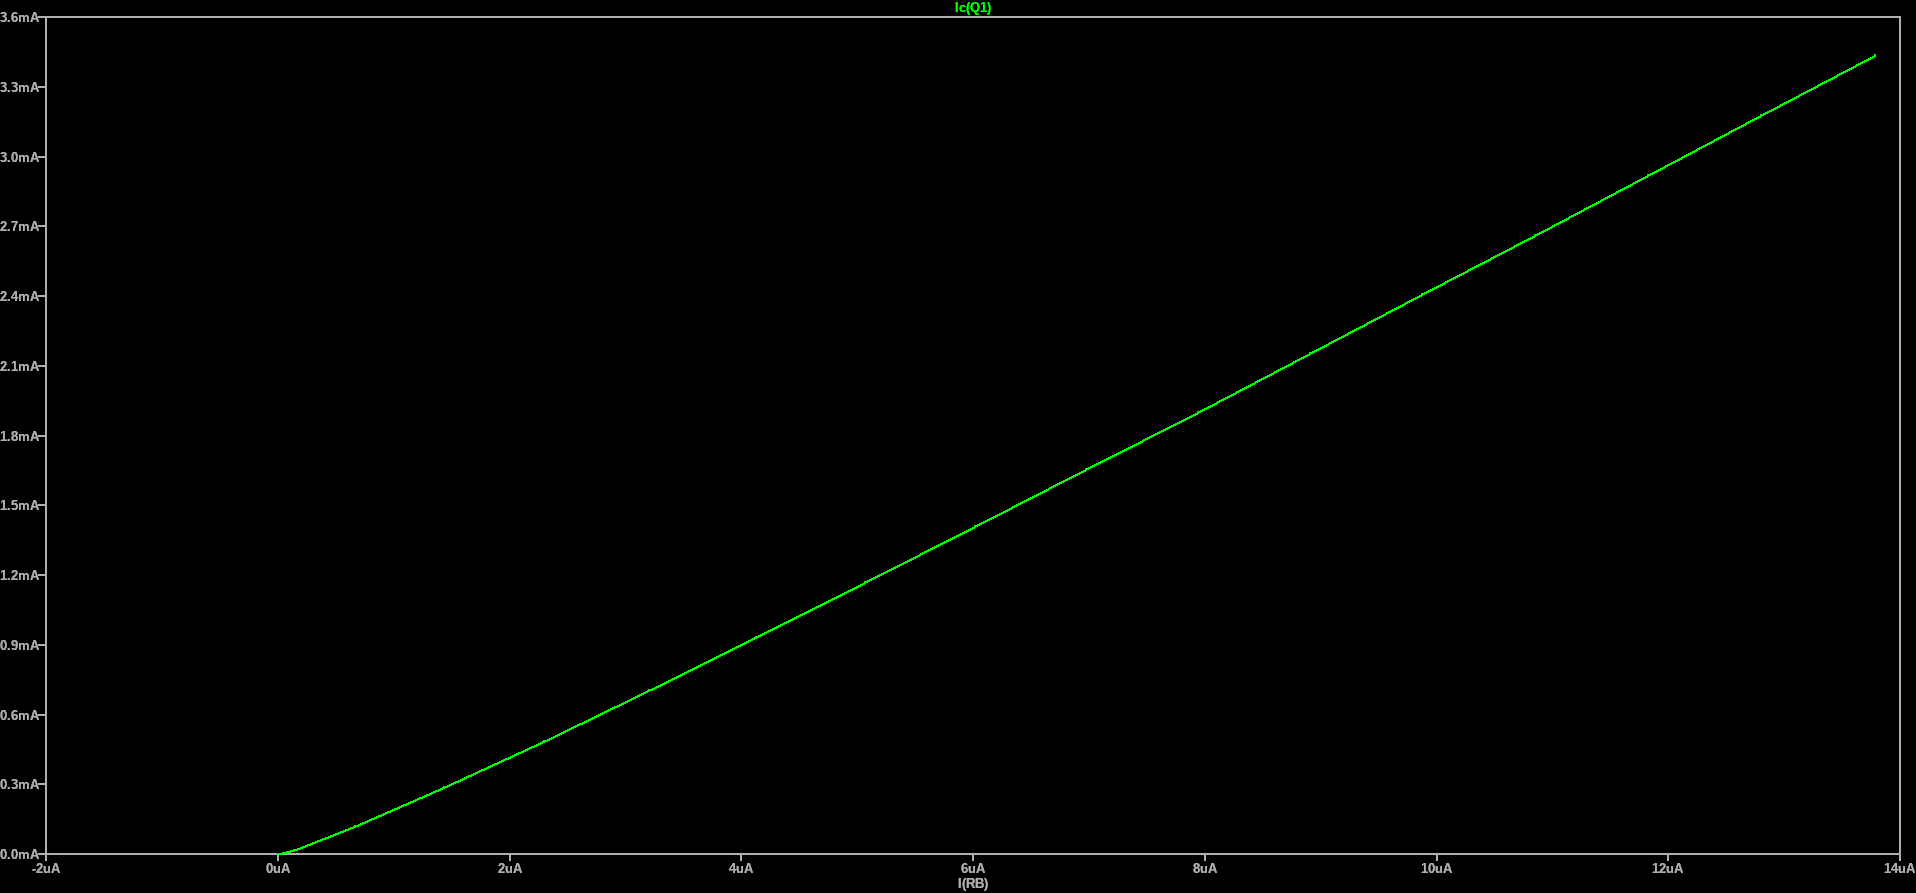
\includegraphics[width=0.4\textwidth]{ProjetBJTEISCPartie1202-img/ProjetBJTEISCPartie1202-img008.png} \\
	Exemple de courbe obtenue
\end{center}

\subsection*{Caractéristique $I_C=f(V_{CE})$}
Pour cela, il faut faire varier la tension entre collecteur et émetteur, ce qu’on peut faire en faisant varier $V_{CC}$ alimenté par $V_2$.

Note : Pour $I_C=f(V_{CE})$ on choisira 3 à 4 valeurs de $I_B$ dans la gamme de compatibilité du transistor.

Pour choisir la plage de courant de base ($I_B$), il faut s’assurer que le point de fonctionnement du transistor ne dépasse jamais les limites destructives définies par le constructeur.

	extbf{Q2.} Tracer l’évolution du gain en courant $\beta = f(I_C)$ (pour $V_{CE}$ fixé) et comparer avec la documentation technique.

	extbf{Q3.} À partir de la caractéristique de transfert en tension $V_{CE}= f(V_{BE})$, tracer l’évolution du gain en tension en fonction du point de polarisation.

\section*{PARTIE 2 : Analyse de cas / conception d’un amplificateur}
Vous décidez de vous lancer dans la conception de l’amplificateur à base du transistor 2SC5876U3 caractérisé dans la partie précédente. Vous travaillez dans un premier temps à vide (sans charge), c'est-à-dire sans connecter le haut-parleur.

Vous testez les différents montages de la figure 2. La simulation devrait aider à comprendre le fonctionnement de ces montages et permettre de comparer avec la théorie.

% Figure 2 : Etude de l’amplificateur à vide
% (Insérer ici la figure 2 si disponible)

% --- Fin du document ---
\end{document}
